\documentclass{IEEEtran} 

%%you can call packages here 
\usepackage[utf8]{inputenc} %utf8 text character encoding
\usepackage{cite}
\usepackage{amsmath,amssymb,amsfonts,nccmath}
\usepackage{hyperref}
\hypersetup{colorlinks,linkcolor={blue},citecolor={blue},urlcolor={red}}  
\usepackage{cleveref} %Para usar crefrange
\usepackage{algorithm,algorithmic}
\usepackage{graphicx}
\usepackage{textcomp}
\usepackage[font=footnotesize,labelfont=bf]{caption}
\usepackage[font=footnotesize,labelfont=bf]{subcaption}
\usepackage{color}
\usepackage{gensymb}
\usepackage{dblfloatfix}
\usepackage{lineno}
\usepackage{enumitem}
\usepackage[autostyle]{csquotes}
\usepackage{latexsym} 


\title{First Practice}
\author{Rodolfo Vera} 


\begin{document}
\maketitle

%%\vspace{-13mm}
\begin{abstract}
     Hola Mundo
\end{abstract}

\section{Introduction} \label{introduction}

Here, we will call for the first cite, reference as \cite{van2014nature}. So, like in \cite{van2014nature,xu2015animal,xu2015animal} we can establish that the animal behaviour, like the random walk can be modelled. Here you can put a general motivation, the problem, related work or state of art, and a general description of the contents of this document.

%%GRAMMARLY 

\section{Objectives}

This is the general objective of the practice
\subsection{Specific objectives or tasks}
Here you can put bullets to put each objective...
\begin{itemize}
\item First task
\item 2nd bullet
	\begin{itemize} 
		\item SubFirst bullet
     \end{itemize}

\item Second task
\end{itemize}

Or if you prefer, you can put numbers like this
\begin{enumerate}
\item One thing
	\begin{enumerate}
		\item One thing
		\item Second Thing
	\end{enumerate}
\item Second Thing
\end{enumerate}

\section{System model or design or how it works }\label{systemModel}
Here you can put the solution to the problem you described in section \ref{introduction}. Use diagrams, flow diagrams, tables, figures, describe the technologies, protocols, standards, methods, algorithms, etc. you are using and why. 
As you can see in the Fig. \ref{thermalmonitoring}, there's a lot of ways you can manipulate the  Figures. 

\begin{figure}[!htbp]
 \centering
		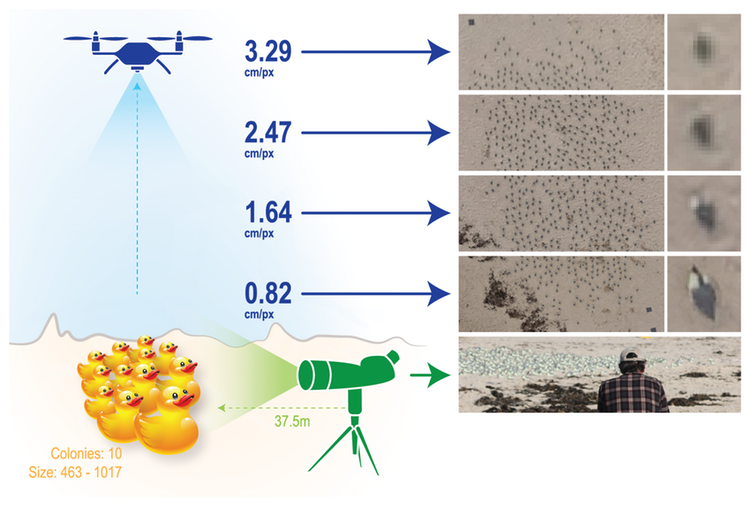
\includegraphics[width=7 cm]{animalmonitoring.png} 
        \caption{Experiment scenario}  
        \label{thermalmonitoring} 
        
\end{figure}  

Besides you can include two subfigures at the same time. like in Fig. \ref{Fig2}. Here you can see that in \cref{thermalmonitoring,thermalmonitoring2,swarm} we are trying to implement a thermal video footage with a Flir camera to study the vital signs of a cattle using a video and a swarm of unmanned aerial vehicles (UAVs). 

\begin{figure}	
 \centering
	\begin{subfigure}{.2\textwidth}
		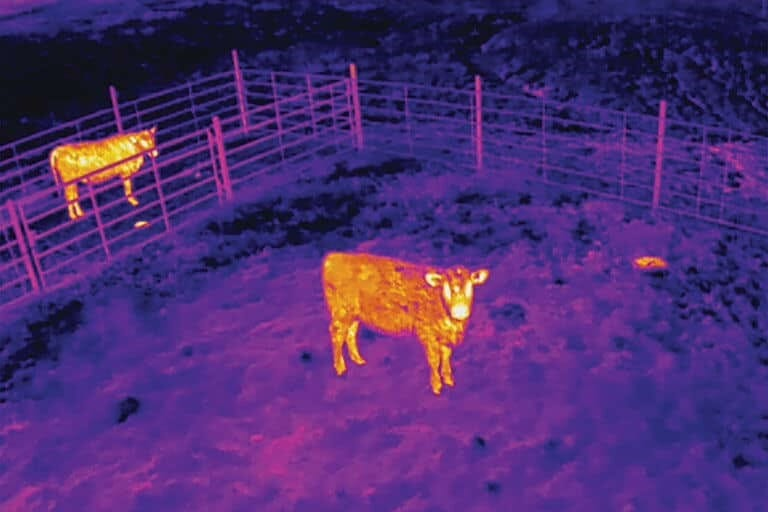
\includegraphics[width=3 cm]{thermalmonitoring.jpg}
        \subcaption{Thermal monitoring 1}
        \label{thermalmonitoring} 
   \end{subfigure}
   \begin{subfigure}{.2\textwidth}
		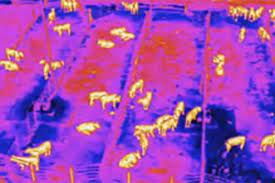
\includegraphics[width=3 cm]{thermalmonitoring2.jpg}
         \subcaption{Thermal monitoring 2}
        \label{thermalmonitoring2} 
   \end{subfigure}  
   \begin{subfigure}{.2\textwidth}
		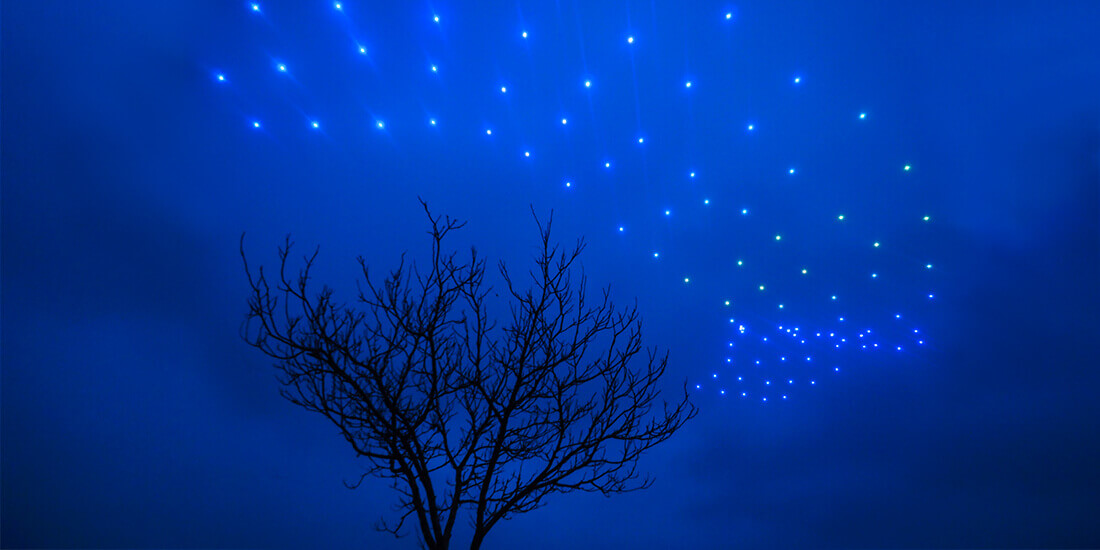
\includegraphics[width=4 cm]{swarm.jpg}
         \subcaption{For swarm }
        \label{swarm} 
   \end{subfigure}  
   \caption{ System implementation of an animal monitoring}
   \label{Fig2}
\end{figure}

then, using the Eq. (\ref{equation1}) we'll able to calculate the velocity of the UAVs when they are flying as 

\begin{equation}\label{equation1}
\nu = \frac{d}{t} 
\end{equation}

where $\nu$ is the velocity, $d$ is for distances in meters and $t$ for time in seconds. On table \ref{table1}, it is described the drone specs. In the following section we will describe the development involve in the making of this work. 

\begin{table}

\caption{UAV Specs}
\centering
\begin{tabular}{| c | c | c | c | }
%\toprule
\hline

\textbf{UAV} & \textbf{Size}	& \textbf{Type} & \textbf{Range}  \\
%\midrule
\hline

 $UAV_1$   & $500\sim$mm	& Quadrotor     & $1000\sim$m
      \\ 
  
 $UAV_2$   & $500\sim$mm	& Quadrotor   & $1000\sim$m        
   \\

 $UAV_3$   & $500\sim$mm	& Quadrotor     & $1000\sim$m        
    \\
%\bottomrule
\hline
\end{tabular}
\label{table1}
\end{table}
\section{Development}
Based on the system model described in section \ref{systemModel}, we develop a system that measures the vital signs of a cattle o 10 cows using Flir technology installed in a swarm of drones. 
\subsection{The Cattle}
The cattle was inside of... 
\subsection{The swarm}
The swarm of UAvs consists on five quadrotors drones, and each drone has the specfications described on table \ref{table1}.
\subsection{Flir camera}
Here the model Flir camera was used and install on every drone... 
\subsection{The monitoring system}
Here, we integrate all ths subsystems, connecting Flir camera to drone through audio video cable and sending the images to GCS with a video transmitter (VT) attacehd to drones. 
 
\section{Results}
Here, you can described the scenario, the tests you made and finally the results, with figs.

\section{Conclusions} 

What did work? what did not? why? What can you fix? What have you learned? and future work, what else can you develop from here?, what can be improved?





\bibliographystyle{ieeetran}

\bibliography{References2}

\end{document}





